\documentclass[11pt]{article}
\usepackage[margin=1in]{geometry}
\usepackage[pdftex]{graphicx}
\usepackage{amsmath,amssymb,amsthm}
\usepackage{lmodern}
\usepackage[T1]{fontenc}
\usepackage{custom}
\usepackage{tikz}
\usetikzlibrary{calc,arrows.meta}

% color boxes
\usepackage[many]{tcolorbox}
\tcbuselibrary{theorems}
\newtcbtheorem{psidea}{Idea}{colback=blue!10,colframe=blue!40!black,fonttitle=\bfseries,breakable,enhanced}{id}
\newtcbtheorem{psremark}{Remark}{colback=purple!10,colframe=purple!40!black,fonttitle=\bfseries,breakable,enhanced}{rm}
\newtcbtheorem{pswrong}{Our version}{colback=orange!10,colframe=orange!50!black,fonttitle=\bfseries,breakable,enhanced}{wr}

% headers and footers
\usepackage{fancyhdr}
\pagestyle{fancy}
\lhead{Gravity from a Spherical Shell}
\chead{}
\rhead{Mechanics}
\lfoot{}
\cfoot{\thepage}
\rfoot{}
\renewcommand{\headrulewidth}{0.4pt}
\setlength{\headheight}{14pt}

\newcommand{\psettitle}[1]{
    \begin{center}
    \huge \textbf{#1}
    \end{center}
}

\linespread{1.03}
\setlength{\parindent}{0.2in}

\begin{document}

\psettitle{Gravity from a Spherical Shell}
\begin{center}
\large The calculation we set up, where the algebra went wrong, and how it finishes
\end{center}

\bigskip

Here's Morin 11.1. A uniform hollow spherical shell has mass $M$ and radius $R$, and a
point mass $m$ sits a distance $r$ from the center. Find the force on $m$, both outside
the shell and inside it, by calculating the potential energy and then differentiating to
get the force.

We set this up together and then lost the thread in the algebra, so here's the same
calculation start to finish, followed by the two lines where ours went off.

\section*{Why potential energy first}

Each little piece of the shell pulls $m$ in a different direction. Adding forces means
adding vectors and keeping track of components, and they're all different. Potential
energy doesn't have a direction. Every piece of the shell contributes $-Gm\,dm/\ell$,
where $\ell$ is that piece's distance from $m$, and you're just adding numbers. Once
you've got $U(r)$, the force comes back out of
\[
F_r = -\frac{dU}{dr}.
\]
That's the same relationship as the one between $U = \tfrac12 k x^2$ and $F = -kx$ for a
spring, which we checked first.

\section*{Slicing the shell into rings}

The useful slice is a \textbf{ring} centered on the line from the shell's center to $m$,
since every point on such a ring is the same distance from $m$. So one number $\ell$
covers the whole ring, and that's what makes a ring the right slice.

\begin{center}
\begin{tabular}{c@{\hspace{0.9cm}}c}
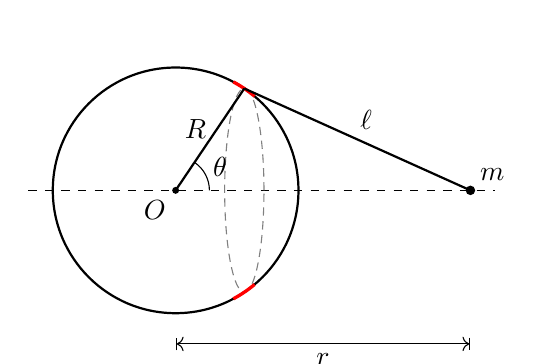
\begin{tikzpicture}[scale=0.78]
  % the shell, seen edge-on
  \draw[thick] (0,0) circle (2);
  \fill (0,0) circle (1.6pt);
  \node[below left] at (0,0) {$O$};

  % axis out to the mass
  \draw[dashed] (-2.4,0) -- (5.2,0);
  \fill (4.8,0) circle (2.2pt);
  \node[above right] at (4.8,0) {$m$};

  % the ring, drawn as an ellipse seen edge-on
  \draw[densely dashed,gray] ({2*cos(56)},0) ellipse ({0.32} and {2*sin(56)});
  \draw[very thick,red] (50:2) arc (50:62:2);
  \draw[very thick,red] (-50:2) arc (-50:-62:2);

  % R, l, theta
  \draw[thick] (0,0) -- (56:2);
  \node at ({1.05*cos(72)},{1.05*sin(72)}) {$R$};
  \draw[thick] (56:2) -- (4.8,0);
  \node at (3.1,1.15) {$\ell$};
  \draw (0.55,0) arc (0:56:0.55);
  \node at ({0.82*cos(28)},{0.82*sin(28)}) {$\theta$};

  % r
  \draw[|<->|] (0,-2.5) -- (4.8,-2.5);
  \node[below] at (2.4,-2.5) {$r$};
\end{tikzpicture}
&
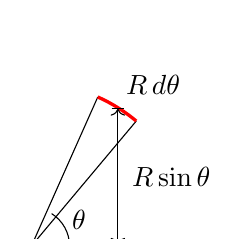
\begin{tikzpicture}[scale=1.15]
  \coordinate (O) at (0,0);
  \draw[dashed] (O) -- (2.1,0);
  \draw (O) -- (50:1.8);
  \draw (O) -- (66:1.8);
  \draw[very thick,red] (50:1.8) arc (50:66:1.8);
  \node[above right] at (59:1.82) {$R\,d\theta$};
  \draw[|<->|] ({1.8*cos(58)},0) -- ({1.8*cos(58)},{1.8*sin(58)});
  \node[right] at ({1.8*cos(58)+0.05},{0.5*1.8*sin(58)}) {$R\sin\theta$};
  \draw (0.42,0) arc (0:58:0.42);
  \node at ({0.6*cos(29)},{0.6*sin(29)}) {$\theta$};
  \fill (O) circle (1.2pt);
\end{tikzpicture}
\end{tabular}
\end{center}

Measure $\theta$ at the center, from the line that runs out toward $m$. The ring between
$\theta$ and $\theta + d\theta$ has radius $R\sin\theta$, so its circumference is
$2\pi R \sin\theta$. Its width, measured along the surface, is $R\,d\theta$, since that's
what a radian means: arc length is radius times angle. Its area is the product:
\[
dA = 2\pi R\sin\theta \cdot R\,d\theta = 2\pi R^2 \sin\theta\,d\theta .
\]

Integrating $dA$ from $\theta = 0$ to $\theta = \pi$ gives $4\pi R^2$, which is a good
sign that we've got the area right. The shell is uniform, so mass follows area:
\[
dm = M\,\frac{dA}{4\pi R^2} = \frac{M}{2}\sin\theta\,d\theta .
\]

The distance from the ring to $m$ comes from the law of cosines, on the triangle with
sides $R$ and $r$ and included angle $\theta$:
\[
\ell = \sqrt{R^2 + r^2 - 2Rr\cos\theta}.
\]

Putting those together and adding up the rings,
\[
U = -\int \frac{Gm\,dm}{\ell}
  = -\frac{GMm}{2}\int_0^{\pi} \frac{\sin\theta\,d\theta}{\sqrt{R^2+r^2-2Rr\cos\theta}} .
\]

\section*{Doing the integral}

Substitute $w = \cos\theta$, so that $dw = -\sin\theta\,d\theta$. At $\theta = 0$ we have
$w = 1$, and at $\theta = \pi$ we have $w = -1$, so the substitution hands the limits back
reversed. The minus sign from $dw$ flips them into the usual order:
\[
U = -\frac{GMm}{2}\int_{-1}^{1} \frac{dw}{\sqrt{R^2+r^2-2Rrw}} .
\]

Now the antiderivative, which is where it's easy to lose a factor of 2. Write
$A = R^2 + r^2$ and $B = 2Rr$, both of which are constants as far as $w$ is concerned.
Differentiating,
\[
\frac{d}{dw}\sqrt{A - Bw} = \frac{-B}{2\sqrt{A-Bw}},
\]
and that $B$ out front is the part that's easy to drop. Running it backwards,
\[
\int \frac{dw}{\sqrt{A-Bw}} = -\frac{2}{B}\sqrt{A-Bw} = -\frac{1}{Rr}\sqrt{A-Bw} .
\]
The chain rule brings the coefficient of $w$ out front, and that coefficient is $2Rr$,
not $1$.

So
\[
U = -\frac{GMm}{2}\cdot\left(-\frac{1}{Rr}\right)\Big[\sqrt{A-Bw}\Big]_{-1}^{1}
  = \frac{GMm}{2Rr}\left(\sqrt{R^2+r^2-2Rr} - \sqrt{R^2+r^2+2Rr}\right).
\]

Both of those square roots are perfect squares:
\[
\sqrt{R^2+r^2+2Rr} = \sqrt{(R+r)^2} = R + r,
\qquad
\sqrt{R^2+r^2-2Rr} = \sqrt{(R-r)^2} = |R-r| .
\]
The absolute value is where the two cases split apart. A square root is never negative,
and $R - r$ is negative whenever $m$ is outside the shell, so you can't just write $R-r$
and move on. The general result is
\[
U = \frac{GMm}{2Rr}\Big(|R-r| - (R+r)\Big),
\]
and now it's just a matter of which side of the shell $m$ is on.

\section*{Outside the shell}

Here $r > R$, so $|R-r| = r - R$ and
\[
U = \frac{GMm}{2Rr}\big((r-R) - (r+R)\big)
  = \frac{GMm}{2Rr}(-2R)
  = -\frac{GMm}{r} .
\]
The radius $R$ has dropped out completely. Differentiating,
\[
F_r = -\frac{dU}{dr} = -\frac{GMm}{r^2},
\]
with the minus sign meaning the force points inward.

\begin{psidea}{The shell theorem, outside}{}
A spherical shell pulls on an outside mass exactly as though all of its mass sat at a
single point at the center. It doesn't matter how big the shell is, as long as $m$ is
outside it.
\end{psidea}

\section*{Inside the shell}

Here $r < R$, so $|R-r| = R - r$ and
\[
U = \frac{GMm}{2Rr}\big((R-r) - (R+r)\big)
  = \frac{GMm}{2Rr}(-2r)
  = -\frac{GMm}{R} .
\]
This time it's $r$ that drops out. The potential energy is the same number everywhere
inside the shell, so
\[
F_r = -\frac{dU}{dr} = 0 .
\]
The force doesn't just get small inside the shell. It's exactly zero, everywhere inside.

The two answers agree at $r = R$, where both give $-GMm/R$, so $U$ is continuous across
the surface even though its slope isn't.

\begin{psremark}{Why the inside cancellation is exact}{}
Stand just inside the shell, with a thin patch of it right under your feet. That patch is
close, so it pulls hard, going like $1/\ell^2$. Look the other way and you see a patch
covering the same solid angle from far across the shell. It pulls more weakly, but it
holds more mass, and its area grows like $\ell^2$. The two effects cancel, and they cancel
exactly only because gravity is an inverse square law. Any other power and you'd feel a
force inside the shell.
\end{psremark}

\section*{Where our version went wrong}

Our setup was right all the way down to
\[
dU = -\frac{GMm}{2}\,\frac{dw}{\sqrt{R^2+r^2-2Rrw}},
\]
and the two square roots we ended up subtracting were right as well. Everything that went
wrong is in the number sitting in front of them.

\begin{pswrong*}{Two lines, two slips}{}
The second-to-last line on our board read
\[
\left[\frac{GMm}{Rr}\sqrt{R^2+r^2-2Rrw}\right]_{-1}^{1},
\qquad\text{where the coefficient should be } \frac{GMm}{2Rr}.
\]
Two different 2's meet at that step: the $\tfrac12$ that came along with
$dm = \tfrac{M}{2}\sin\theta\,d\theta$, and the $2Rr$ that the chain rule brings down.
Only one of them survived, so that line is already a factor of $2$ too big.

Then the last line came out as
\[
\frac{2GMm}{Rr}\left(\sqrt{R^2+r^2+2Rr}-\sqrt{R^2+r^2-2Rr}\right) = \frac{4GMm}{r} .
\]
The two square roots have traded places between those lines, which flips the sign, and
another factor of $2$ has appeared out front. Our answer came out $-4$ times the right
one.
\end{pswrong*}

The warm-up we wrote off to the side,
\[
\frac{d}{dx}\sqrt{1-x} = -\frac{1}{2\sqrt{1-x}},
\]
is correct, but it's the special case where the coefficient of $x$ happens to be $1$.
Carrying it straight across to $\sqrt{A - Bw}$ is what let the factors of $2$ wander.
Whenever a substitution leaves a constant sitting next to the variable, it's a good idea
to name it, the way we named $B$ above, so the chain rule has something visible to act on.

Two quick checks catch this. The first is the sign. With the zero of potential energy set
at infinite separation, gravitational potential energy is negative everywhere, so a
positive answer is wrong before you look at anything else. The second is to shrink the
shell: let $R \to 0$ and it becomes an ordinary point mass, so $U$ has to come out to
exactly $-GMm/r$. Ours gave $+4GMm/r$, which has the right dimensions and the right
dependence on $r$, and that's why it looked plausible. But it's four times too big, and it
points the wrong way.

\section*{What the result buys you}

A solid sphere, or any body whose density depends only on distance from the center, is a
stack of shells. For a mass at distance $r$ from the center, every shell inside that
radius pulls as though its mass were at the center, and every shell outside it pulls not
at all. Only the enclosed mass matters:
\[
F = \frac{G M_{\text{enc}}(r)\,m}{r^2} .
\]
For a uniform sphere, $M_{\text{enc}} = M r^3/R^3$, so $g$ rises linearly from zero at the
center to $GM/R^2$ at the surface and falls off as $1/r^2$ beyond. That's the plot we
sketched.

This is also why you can treat the Earth and the Moon as points when you write down
$GMm/r^2$, which isn't obvious, and which Newton had to prove before the rest of his
gravitation could stand. The integral above is roughly what it cost him.

\end{document}
